% tags: arc edgeLabel label blockDiagram house background align
\PassOptionsToPackage{usenames,dvipsnames}{xcolor}
\documentclass[tikz, border=10pt]{standalone}

\usepackage{verbatim}
\usepackage{amsmath}

\tikzset{>=stealth}
\tikzstyle{every node}=[align=center]
\usetikzlibrary{spy,shadows,arrows,shapes,positioning,calc,backgrounds,fit,automata}

\newcommand{\Green}{OliveGreen!40}
\newcommand{\Yellow}{GreenYellow!70}
\newcommand{\Orange}{Orange!60}
\newcommand{\Brown}{Sepia!40}
\newcommand{\DarkGreen}{OliveGreen!60}
\newcommand{\DarkOrange}{Orange}
\newcommand{\DarkYellow}{GreenYellow!120}
\newcommand{\DarkBrown}{Sepia!60}
\begin{document}
\pgfdeclarelayer{bg}
\pgfdeclarelayer{fg}
\pgfsetlayers{bg,main,fg}
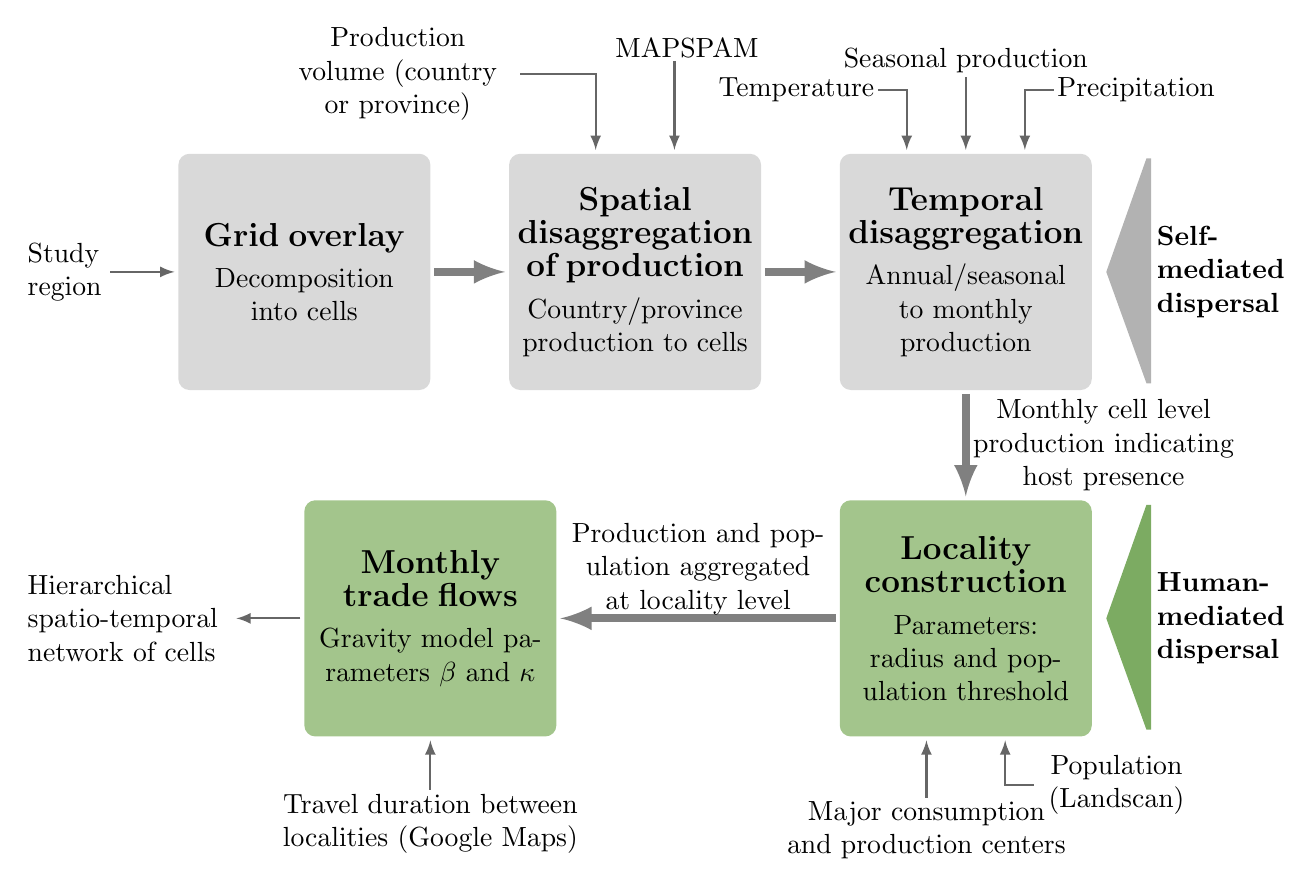
\begin{tikzpicture}
    [blk/.style={inner sep=.1cm,fill=black!15,rounded corners,text width=3cm,minimum height=3cm},
every node/.style={inner sep=0,align=center},
blkedge/.style={draw=black!50,>=latex, shorten >=1pt, shorten <=1pt, line
width=1mm},
datedge/.style={draw,>=latex, draw=black!60, shorten >=1pt, shorten <=1pt},
node distance=4.2cm,thick]

%% grid
\node[blk,fill=black!15] (grid) {\textbf{\large Grid overlay}\\\smallskip Decomposition into cells};
\draw[datedge,<-] (grid) -- +(-2.5cm,0) node[shift={(-.2,0)},inner
sep=0,text width=.8cm,anchor=east,align=left]{Study \\ region};
%% spatial
\node[blk,fill=black!15,right of=grid] (spatial) {\textbf{\large Spatial \\ disaggregation of
production} \\ \smallskip Country/province production to cells};
\draw[blkedge,->] (grid) -- (spatial);
\draw[datedge,<-] ($(spatial.north)+(-.5,0)$) |- +(-1cm,1cm) node[text
width=3cm,anchor=east] {Production volume (country or province)};
\draw[datedge,<-] ($(spatial.north)+(+.5,0)$) -- +(0cm,1.2cm) node[text
width=1.5cm,anchor=south] {MAPSPAM};
%% temporal
\node[blk,fill=black!15,right of=spatial] (temporal) {\textbf{\large Temporal
    disaggregation} \\
\smallskip Annual/seasonal to monthly production};
\draw[blkedge,->] (spatial) -- (temporal);
\draw[datedge,<-] ($(temporal.north)+(-.75,0)$) |- +(-.4cm,.8cm)
node[anchor=east] {Temperature};
\draw[datedge,<-] ($(temporal.north)+(0,0)$) -- +(0cm,1cm)
node[anchor=south] {Seasonal production};
\draw[datedge,<-] ($(temporal.north)+(.75,0)$) |- +(.4cm,.8cm)
node[anchor=west] {Precipitation};
%% locality
\node[blk,fill=\Green,below of=temporal,shift={(0,-.2)}] (locality) {\textbf{\large Locality
construction} \\\smallskip Parameters: radius and population threshold};
\draw[blkedge,->] (temporal) -- node [text width=3.4cm,anchor=west] {Monthly
cell level production indicating host presence} (locality);
\draw[datedge,<-] ($(locality.south)+(.5,0)$) |- +(.4cm,-.6cm)
node[text width=2cm,anchor=west] {Population (Landscan)};
\draw[datedge,<-] ($(locality.south)+(-.5,0)$) -- +(0cm,-.8cm)
node[text width=5cm,anchor=north] {Major consumption and production centers};
%% gravity
\node[blk,fill=\Green,left of=locality,shift={(-2.6,0)}] (gravity) {\textbf{\large Monthly trade flows
}\\\smallskip Gravity model parameters $\beta$ and $\kappa$};
\draw[blkedge,->] (locality) -- (gravity) node[midway,text width=3.3cm,anchor=south]
{Production and population aggregated at locality level};
\draw[datedge,<-] ($(gravity.south)+(0,0)$) -- +(0cm,-.7cm)
node[text width=5cm,anchor=north] {Travel duration between localities (Google Maps)};
%% final
\draw[datedge,->] (gravity) -- +(-2.5,0) node[align=left,inner
sep=0,shift={(-.1,0)},anchor=east,text width=2.5cm]
{{Hierarchical spatio-temporal network of cells}};
%%
%% \begin{pgfonlayer}{bg}
%% \draw[draw=\Red,ultra thick] ($(grid.north
%% west)+(-.1,.1)$) rectangle ($(temporal.south east)+(.1,-.1)$);
%% %% \draw[\Red,ultra thick] ($(temporal.north east)+(.1,.1)$) -- +(.4,0)
%% %% arc(90:-90:1.6) -- +(-.4,0);
%% %% \draw[\DarkRed,ultra thick] ($(temporal.east)+(.2,0)$) --
%% %% ($(temporal.north east)+(1,.1)$) node (anch) {} -- ++(1.3,0) -- ++(0,-3.2)
%% %% -- ($(anch)+(0,-3.2)$) -- cycle;
\draw[black!30,fill=black!30,ultra thick] ($(temporal.east)+(.2,0)$) --
($(temporal.north east)+(.7,-.1)$) node (anch) {} -- ++(.01,0) -- ++(0,-2.8)
-- ($(anch)+(0,-2.8)$) -- cycle;
%% %% \draw[\DarkRed,ultra thick] ($(temporal.east)+(.2,0)$) --
%% %% ($(temporal.north east)+(.7,-.2)$) -- ++(0,-2.6) -- cycle;
%% \draw[draw=\Blue,ultra thick] ($(gravity.north
%% west)+(-.1,.1)$) rectangle ($(locality.south east)+(.1,-.1)$);
%% %% \draw[\DarkBlue,ultra thick] ($(locality.east)+(.2,0)$) --
%% %% ($(locality.north east)+(1,.1)$) node (anch) {} -- ++(1.3,0) -- ++(0,-3.2)
%% %% -- ($(anch)+(0,-3.2)$) -- cycle;
\draw[\DarkGreen,fill=\DarkGreen,ultra thick] ($(locality.east)+(.2,0)$) --
($(locality.north east)+(.7,-.1)$) node (anch) {} -- ++(.01,0) -- ++(0,-2.8)
-- ($(anch)+(0,-2.8)$) -- cycle;
%% \end{pgfonlayer}
\node at (temporal.east) [inner sep=0cm,anchor=west,text
width=1.56cm,text =black,shift={(.8,0)},align=left] {\bfseries Self-mediated dispersal};
\node at (locality.east) [inner sep=0cm,anchor=west,text
width=1.56cm,shift={(.8,0)},align=left] {\bfseries Human-mediated dispersal};
\end{tikzpicture}
\end{document}
